\documentclass[12pt]{article}
\usepackage[utf8]{inputenc}
\usepackage[spanish]{babel}
\usepackage{graphicx}
\usepackage{amsmath}
\usepackage{amssymb}
\usepackage{hyperref}
\usepackage{geometry}
\usepackage{float}
\usepackage{booktabs}
\usepackage{caption}
\usepackage{subcaption}
\usepackage{cite}

\geometry{a4paper, margin=2.5cm}

\title{Optimización Multi-Objetivo en Deep Learning Físicamente Informado para la Caracterización de Dominios Magnéticos Nanoscópicos}

\author{Juan Sebastián Méndez Rondón\\
Universidad Nacional de Colombia - Sede Manizales\\
Materia: Optimización}

\date{\today}

\begin{document}

\maketitle

\begin{abstract}
Este trabajo aborda un problema de optimización multi-objetivo en el contexto del proyecto doctoral ``Explainable Deep Learning Framework for estimating and generating Magnetic Domains from hamiltonian parameters''. Se presenta la caracterización de dominios magnéticos nanoscópicos mediante modelos generativos profundos condicionados por parámetros físicos del Hamiltoniano. El problema central consiste en optimizar simultáneamente múltiples términos conflictivos en la función de pérdida de un modelo cVAE (Conditional Variational Autoencoder) combinado con regularización física y redes generativas adversarias (GANs), donde la mejora en la reconstrucción de imágenes puede deteriorar la capacidad generativa, y viceversa. Se describe la formulación del problema multi-objetivo, la metodología propuesta y los experimentos realizados hasta la fecha.
\end{abstract}

\section{Introducción y Vinculación con Optimización}

Este documento se desarrolla en el marco de la materia de Optimización del programa de doctorado en Ingeniería de la Universidad Nacional de Colombia, Sede Manizales. El trabajo presenta un caso de estudio práctico de optimización multi-objetivo aplicado a uno de los problemas centrales del proyecto doctoral: la mitigación de la degeneración de estados magnéticos mediante el ajuste de hiperparámetros en modelos de deep learning físicamente informados.

La degeneración de estados magnéticos se refiere al fenómeno por el cual múltiples configuraciones de espines microscópicos pueden corresponder a los mismos valores de parámetros macroscópicos del Hamiltoniano (temperatura, interacciones de intercambio, anisotropía, etc.). Este problema de no-unicidad en el mapeo inverso (parámetros $\to$ configuraciones) dificulta tanto la estimación de parámetros físicos a partir de imágenes experimentales como la generación de configuraciones realistas a partir de condiciones físicas conocidas.

La solución propuesta emplea un modelo generativo condicional (cVAE) que aprende una distribución latente condicionada por parámetros físicos, combinado con restricciones de regularización física (penalidades de energía micromagnética, residuales de Landau-Lifshitz-Gilbert) y técnicas adversarias (GANs) para mejorar la calidad visual de las imágenes generadas. Sin embargo, estos componentes introducen términos conflictivos en la función objetivo, convirtiendo el entrenamiento del modelo en un problema de optimización multi-objetivo donde no existe una solución óptima única, sino un conjunto de soluciones Pareto-eficientes.

\section{Temática: Dominios Magnéticos Nanoscópicos}

\subsection{¿Qué son los dominios magnéticos?}

Los dominios magnéticos son regiones microscópicas en materiales ferromagnéticos donde los momentos magnéticos atómicos (espines) están alineados en una dirección común. La formación de estos dominios minimiza la energía magnetostática total del sistema. Las paredes de dominio—regiones de transición entre dominios con orientaciones diferentes—juegan un papel crucial en las propiedades magnéticas macroscópicas del material.

\begin{figure}[H]
    \centering
    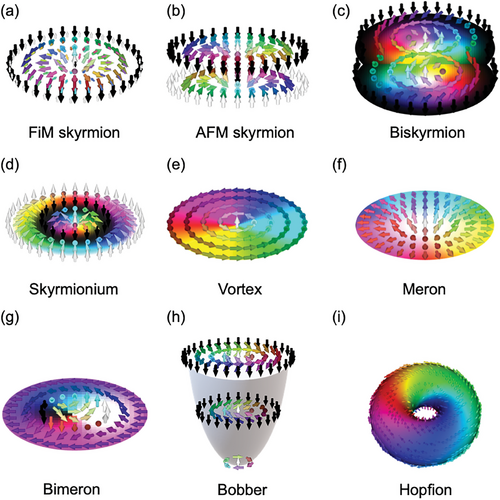
\includegraphics[width=0.7\textwidth]{Figures/magneticTexture.jpg}
    \caption{Ejemplo de texturas magnéticas complejas observadas en materiales nanoscópicos. Estas configuraciones incluyen vórtices magnéticos, skyrmiones, y paredes de dominio con topologías no triviales.}
    \label{fig:magnetic_texture}
\end{figure}

A escala nanométrica, los dominios magnéticos exhiben texturas complejas como skyrmiones (cuasipartículas topológicas), vórtices magnéticos, y estructuras quirales inducidas por la interacción de Dzyaloshinskii-Moriya (DMI). Estas configuraciones son de gran interés para aplicaciones en espintrónica, dispositivos de memoria magnética de alta densidad (MRAM), y computación neuromorfa.

\subsection{Motivación}

La caracterización precisa de dominios magnéticos nanoscópicos presenta desafíos fundamentales que limitan tanto el entendimiento físico como las aplicaciones tecnológicas:

\begin{enumerate}
    \item \textbf{Dificultad experimental}: Las técnicas de microscopía (MFM, LTEM, SP-STM) producen imágenes con ruido, artefactos, y resolución limitada. La adquisición de datos experimentales de alta calidad es costosa y consume tiempo considerable.

    \item \textbf{Complejidad computacional de simulaciones}: Los métodos micromagnéticos (MuMax3, OOMMF) y simulaciones atomísticas Monte Carlo son computacionalmente costosos, requiriendo horas o días para generar configuraciones de equilibrio térmico.

    \item \textbf{Degeneración de parámetros}: Múltiples conjuntos de parámetros del Hamiltoniano pueden producir configuraciones magnéticas visualmente similares, dificultando el problema inverso de estimar parámetros físicos a partir de observaciones experimentales.

    \item \textbf{Falta de interpretabilidad}: Los modelos de deep learning aplicados a este dominio funcionan como ``cajas negras'', sin garantizar que las predicciones sean físicamente plausibles o consistentes con las leyes fundamentales del magnetismo.
\end{enumerate}

\begin{figure}[H]
    \centering
    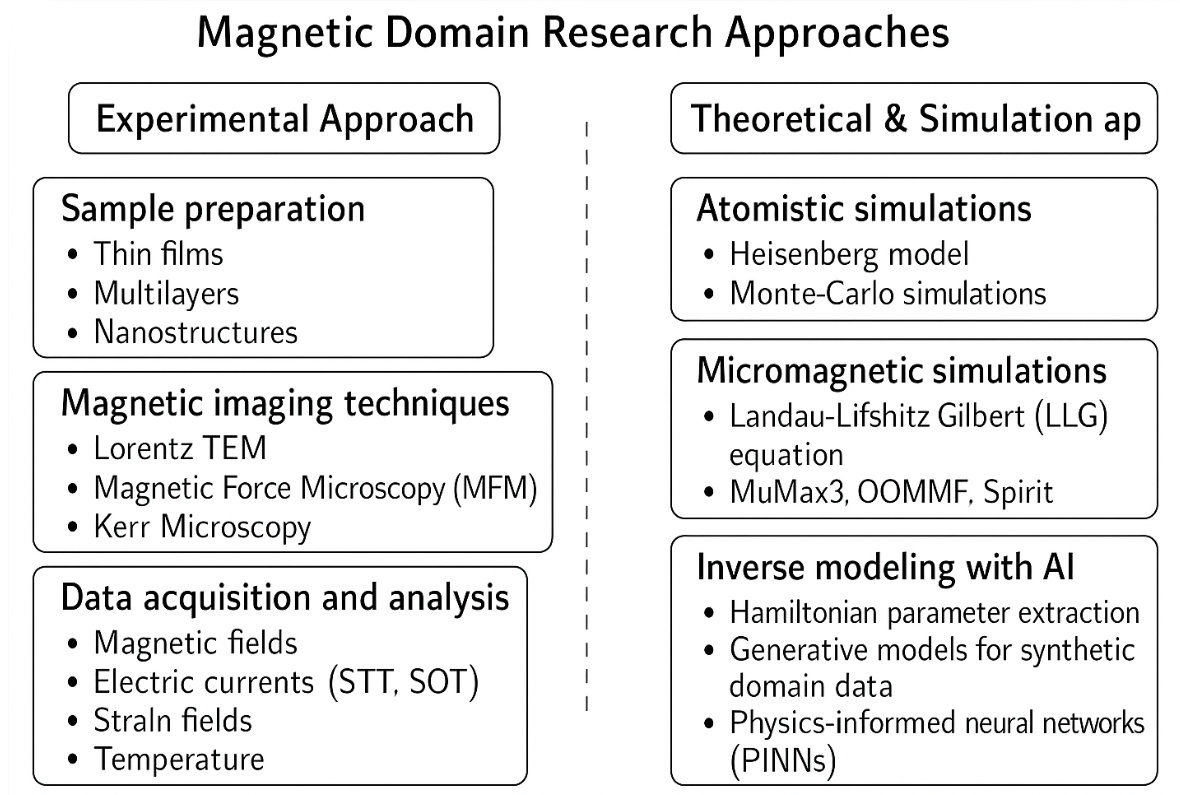
\includegraphics[width=0.95\textwidth]{Figures/ProblemStatement.png}
    \caption{Visión general de los desafíos en la caracterización de dominios magnéticos: la brecha entre simulaciones de alta fidelidad (costosas), datos experimentales de baja calidad, y la necesidad de modelos interpretables que respeten principios físicos.}
    \label{fig:problem_statement}
\end{figure}

\section{Problem Statements}

El proyecto doctoral aborda tres problemas complementarios en la modelación de dominios magnéticos mediante deep learning físicamente informado. Cada problema se formula como una tarea de optimización con restricciones físicas y regularizaciones específicas.

\subsection{Problema 1: Degeneración de Estados Magnéticos y Optimización Multi-Objetivo}

\textbf{Formulación del problema}: Dado un conjunto de parámetros del Hamiltoniano $\mathbf{c} = \{T, J_{ex}, K_{an}, D_{DM}, H_{ext}, \ldots\}$ que describen las condiciones físicas de un sistema magnético, el objetivo es generar una distribución de configuraciones de espines $p(x|\mathbf{c})$ que:

\begin{enumerate}
    \item Sean consistentes con las restricciones impuestas por $\mathbf{c}$
    \item Minimicen el funcional de energía micromagnética $E[x; \mathbf{c}]$
    \item Sean visualmente plausibles y libres de artefactos no físicos
    \item Capturen la variabilidad natural debida a fluctuaciones térmicas y estados metaestables
\end{enumerate}

\begin{figure}[H]
    \centering
    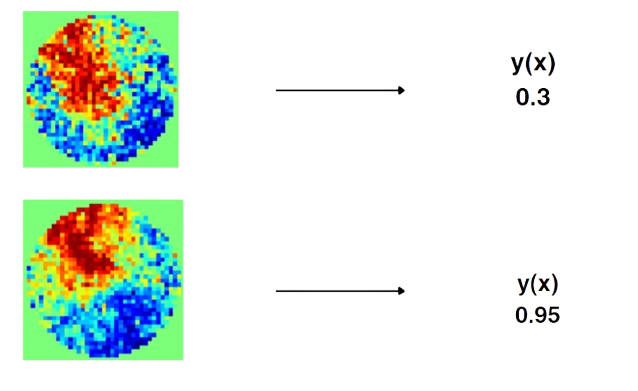
\includegraphics[width=0.9\textwidth]{Figures/Problems1.png}
    \caption{Problema 1 - Degeneración de estados: múltiples configuraciones magnéticas visualmente distintas pueden corresponder a los mismos parámetros del Hamiltoniano, especialmente cerca de transiciones de fase o en presencia de frustración magnética.}
    \label{fig:problem1}
\end{figure}

\textbf{Naturaleza multi-objetivo}: Este problema no admite una solución óptima única, sino un conjunto de soluciones Pareto-eficientes donde mejorar un objetivo deteriora necesariamente otro. Los objetivos en conflicto son:

\begin{itemize}
    \item \textbf{Fidelidad de reconstrucción} ($\mathcal{L}_{recon}$): Minimizar el error entre configuraciones reales y reconstruidas (MSE a nivel de píxel)
    \item \textbf{Regularización KL} ($\mathcal{L}_{KL}$): Mantener la distribución latente cercana al prior aprendido para garantizar capacidad generativa
    \item \textbf{Consistencia física} ($\mathcal{L}_{phys}$): Minimizar la energía micromagnética y los residuales de la ecuación de Landau-Lifshitz-Gilbert
    \item \textbf{Calidad perceptual} ($\mathcal{L}_{GAN}$): Generar configuraciones visualmente indistinguibles de datos reales según un discriminador adversario
\end{itemize}

La función de pérdida total es una combinación ponderada:

\begin{equation}
\mathcal{L}_{total} = \alpha \mathcal{L}_{recon} + \beta \mathcal{L}_{KL} + \gamma \mathcal{L}_{phys} + \delta \mathcal{L}_{GAN}
\end{equation}

donde los hiperparámetros $\{\alpha, \beta, \gamma, \delta\}$ determinan el trade-off entre objetivos. El problema de optimización consiste en encontrar valores óptimos de estos pesos junto con los parámetros de las redes neuronales $\{\theta_{enc}, \theta_{dec}, \theta_{prior}, \theta_{disc}\}$.

\textbf{Interacciones entre objetivos}:

\begin{enumerate}
    \item \textbf{$\mathcal{L}_{recon}$ vs $\mathcal{L}_{KL}$}: Aumentar $\beta$ mejora la capacidad generativa (muestras más diversas del prior) pero deteriora la precisión de reconstrucción punto a punto. Reducir $\beta$ produce reconstrucciones perfectas pero colapsa la distribución latente a un delta de Dirac, eliminando la capacidad generativa.

    \item \textbf{$\mathcal{L}_{phys}$ vs $\mathcal{L}_{recon}$}: Las penalidades de energía física fuerzan configuraciones de baja energía, pero las imágenes reales pueden contener estados metaestables de alta energía capturados experimentalmente. Un $\gamma$ alto sesga el modelo hacia configuraciones de equilibrio térmico, perdiendo diversidad.

    \item \textbf{$\mathcal{L}_{GAN}$ vs $\mathcal{L}_{KL}$}: El discriminador adversario penaliza imágenes que no parecen ``reales'', favoreciendo configuraciones que coinciden con la distribución empírica. Esto puede entrar en conflicto con la regularización KL que busca mantener una distribución latente gaussiana suave.

    \item \textbf{Hiperparámetros de red}: La dimensión latente $d$, la tasa de aprendizaje, la profundidad de las redes, y el número de épocas también afectan el balance entre objetivos de manera no trivial.
\end{enumerate}

\subsection{Problema 2: Calidad de Datos Experimentales}

Las imágenes experimentales de dominios magnéticos sufren de:
\begin{itemize}
    \item Ruido instrumental (térmico, electrónico)
    \item Artefactos de adquisición (distorsión geométrica, efectos de punta en MFM)
    \item Resolución limitada (difuminado, pérdida de detalles finos)
    \item Escasez de datos etiquetados de alta calidad
\end{itemize}

\textbf{Objetivo}: Desarrollar técnicas de adaptación de dominio (domain adaptation) y mejoramiento de calidad (super-resolución, denoising) para transferir conocimiento desde simulaciones de alta fidelidad hacia datos experimentales ruidosos, preservando la consistencia física.

\subsection{Problema 3: Interpretabilidad de Modelos}

Los modelos de deep learning entrenados de manera puramente empírica (end-to-end) carecen de garantías sobre:
\begin{itemize}
    \item Plausibilidad física de predicciones
    \item Generalización fuera de distribución (out-of-distribution)
    \item Identificabilidad de parámetros físicos
\end{itemize}

\textbf{Objetivo}: Incorporar conocimiento físico explícito (leyes de conservación, simetrías, funcionales de energía) directamente en la arquitectura y función de pérdida, desarrollando métodos de interpretabilidad que relacionen activaciones de la red con características físicas relevantes (paredes de dominio, vórtices, defectos topológicos).

\section{Metodología Propuesta}

La metodología integra cuatro componentes diseñados para trabajar de manera sinérgica, cada uno abordando aspectos específicos de los problemas planteados.

\subsection{Autoencoder Variacional Condicional con Priors Físicamente Guiados (cVAE)}

A diferencia de los VAEs clásicos que imponen un prior fijo $p(z) = \mathcal{N}(0, I)$, el modelo propuesto aprende un prior condicional dependiente de los parámetros físicos:

\begin{equation}
p_\psi(z|\mathbf{c}) = \mathcal{N}(\mu_\psi(\mathbf{c}), \Sigma_\psi(\mathbf{c}))
\end{equation}

donde $\psi$ son los parámetros de una red neuronal (Prior Network) que mapea las condiciones físicas $\mathbf{c}$ a la media y varianza del prior latente.

\begin{figure}[H]
    \centering
    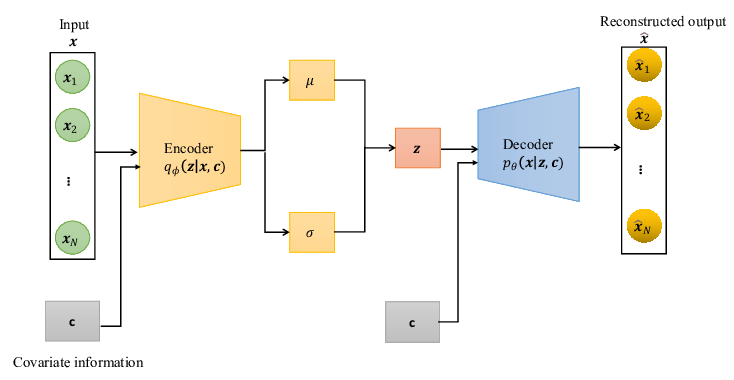
\includegraphics[width=0.85\textwidth]{Figures/cVae.png}
    \caption{Arquitectura del cVAE con prior condicional aprendido. El Prior Network $P_\psi$ estructura el espacio latente según parámetros físicos, mientras el encoder $Q_\phi$ y decoder $G_\theta$ realizan la codificación y reconstrucción condicionadas.}
    \label{fig:cvae_arch}
\end{figure}

\textbf{Función de pérdida base}:

\begin{equation}
\mathcal{L}_{VAE} = \mathbb{E}_{q_\phi(z|x,\mathbf{c})}\left[\log p_\theta(x|z,\mathbf{c})\right] - \beta \, D_{KL}\left[q_\phi(z|x,\mathbf{c}) \,\|\, p_\psi(z|\mathbf{c})\right]
\end{equation}

El primer término mide la fidelidad de reconstrucción, mientras el segundo regulariza la distribución del encoder hacia el prior condicional aprendido. El hiperparámetro $\beta$ controla el balance entre ambos objetivos (conocido como $\beta$-VAE).

\subsection{Framework Ciclo-Consistente Forward-Inverse}

Para reducir la degeneración de parámetros, se acopla el generador forward (parámetros $\to$ configuraciones) con un estimador inverso (configuraciones $\to$ parámetros):

\begin{equation}
\mathcal{L}_{cycle} = \left\|\mathbf{c} - f_{inv}(f_{fwd}(\mathbf{c}))\right\|^2 + \left\|x - f_{fwd}(f_{inv}(x))\right\|^2
\end{equation}

Esta restricción de ciclo-consistencia impone que:
\begin{itemize}
    \item Una configuración generada desde $\mathbf{c}$ debe producir la estimación $\hat{\mathbf{c}} \approx \mathbf{c}$ cuando se pasa por el estimador inverso
    \item Una configuración real $x$ debe ser reconstruida consistentemente tras el ciclo completo
\end{itemize}

\begin{figure}[H]
    \centering
    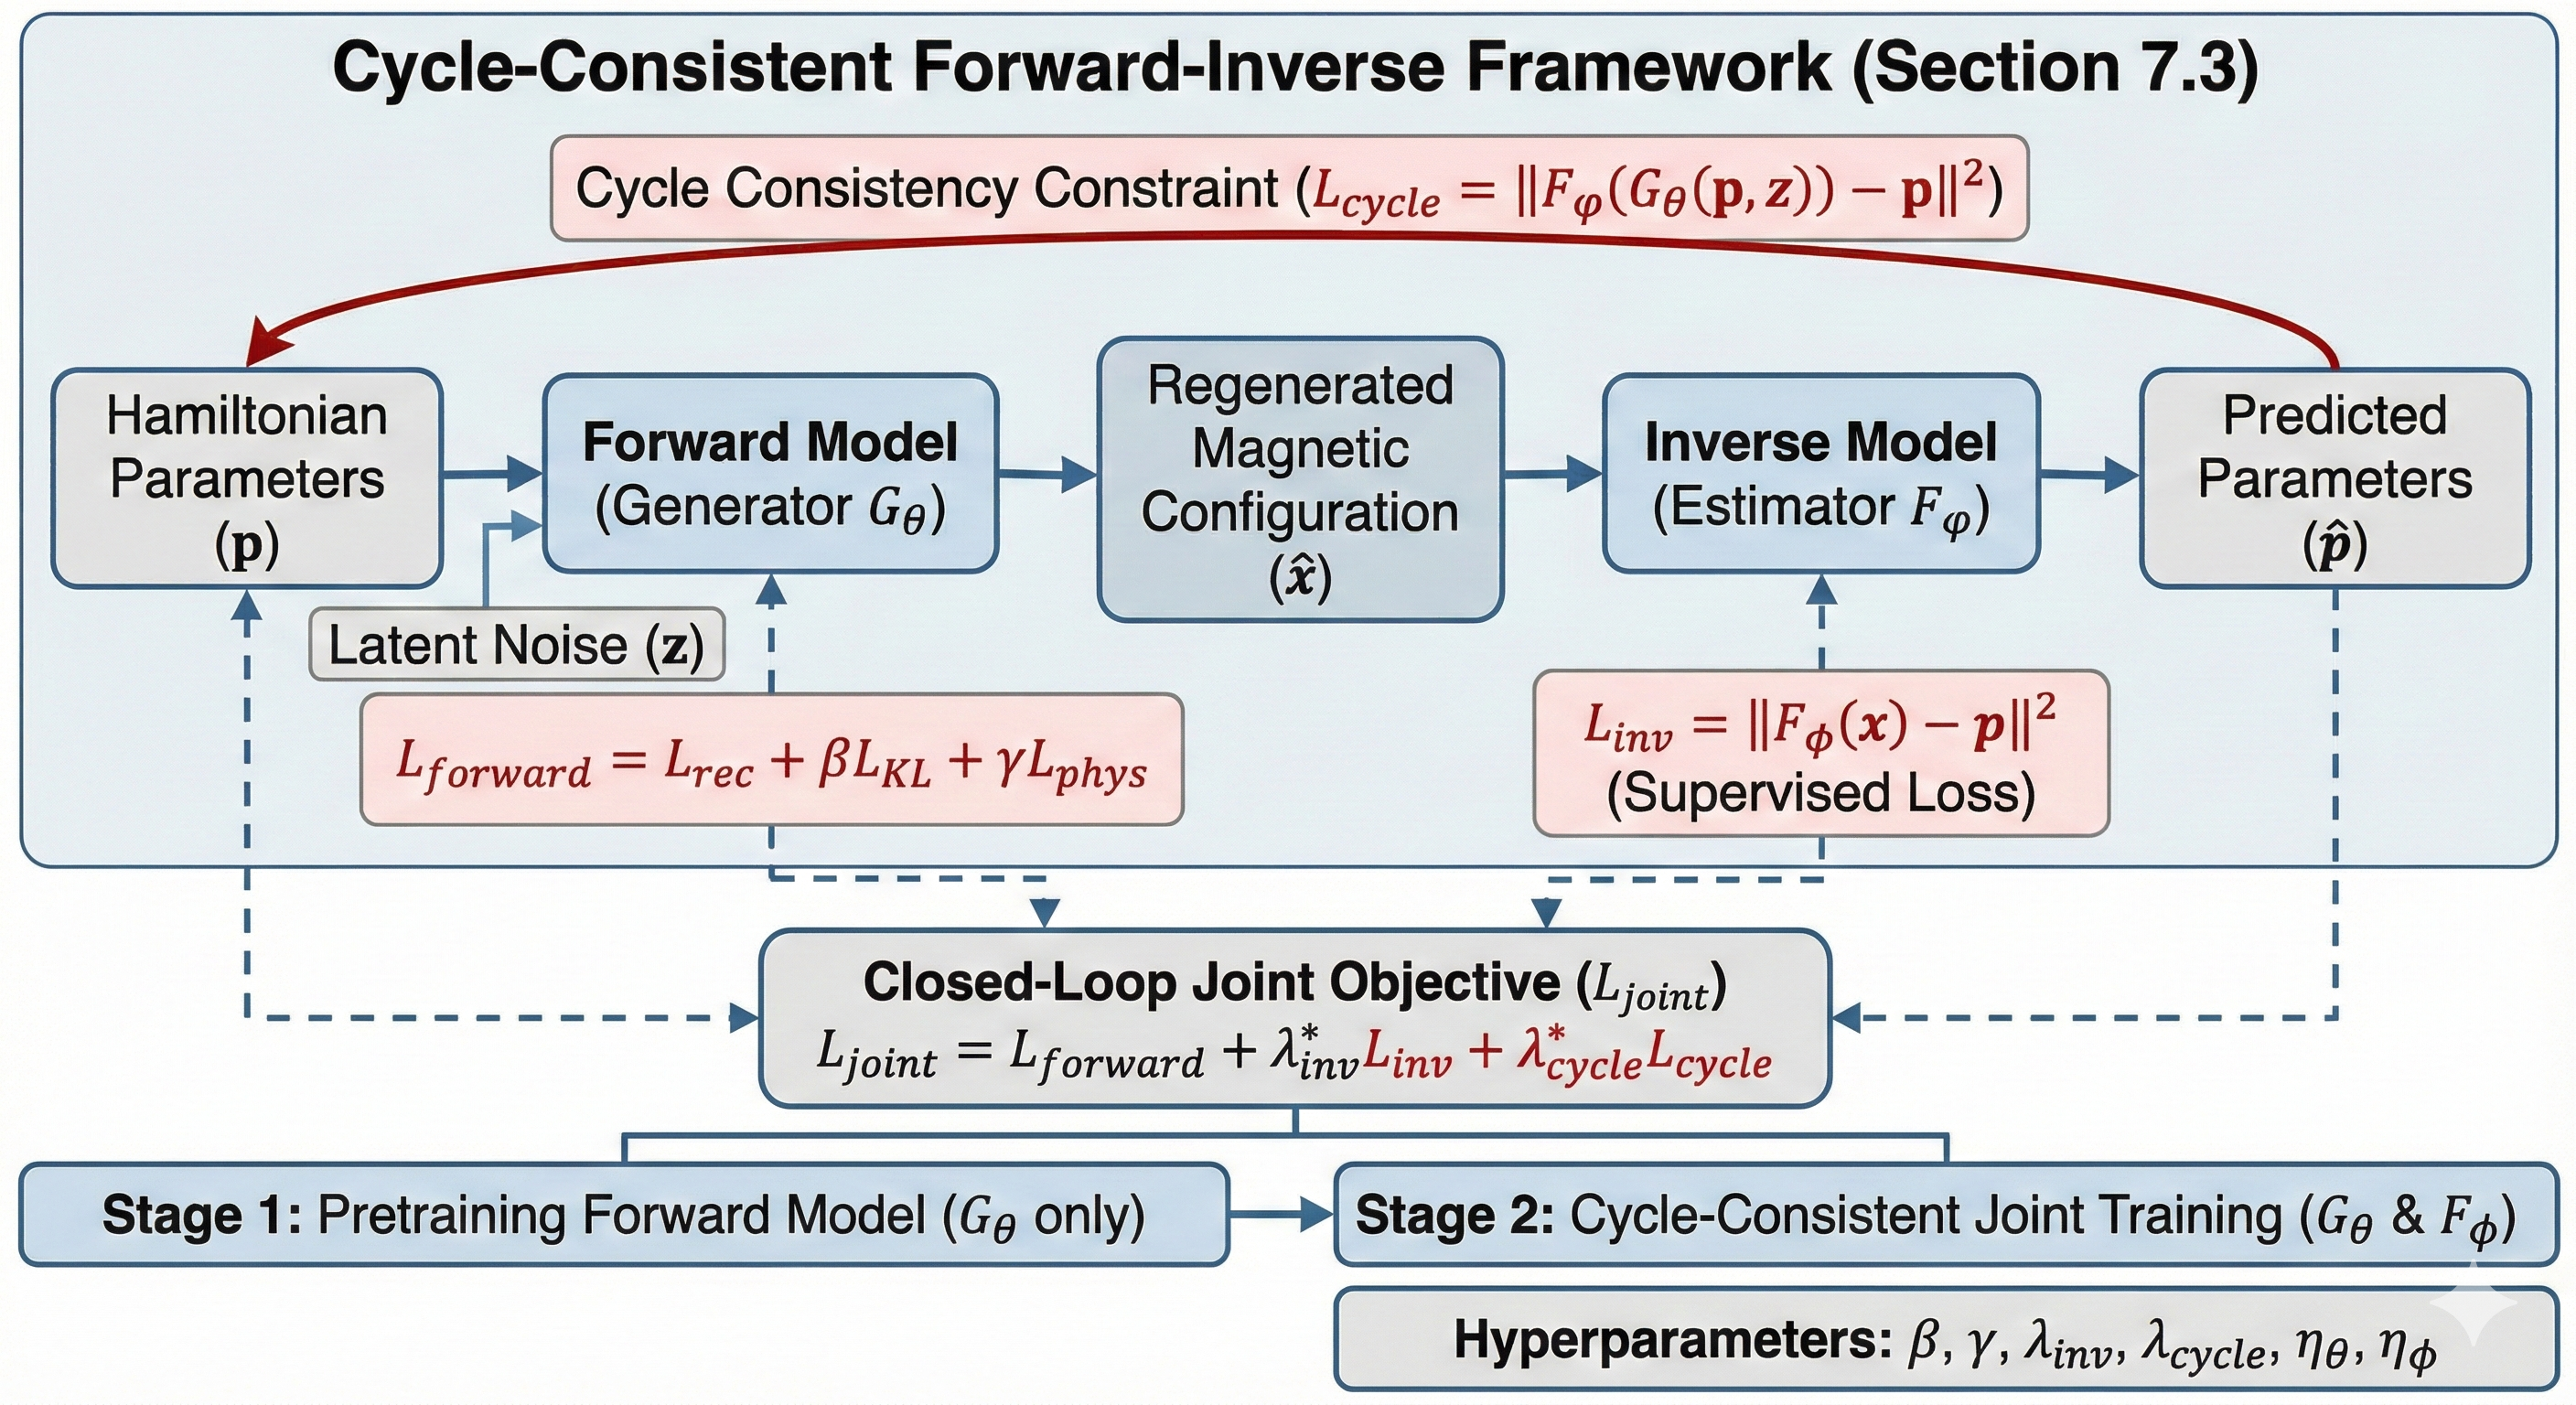
\includegraphics[width=0.9\textwidth]{Figures/Cycle.png}
    \caption{Framework ciclo-consistente: el flujo forward genera configuraciones desde parámetros, y el flujo inverse estima parámetros desde configuraciones. Las restricciones de ciclo fuerzan consistencia bidireccional.}
    \label{fig:cycle}
\end{figure}

\subsection{Regularización Físicamente Informada}

Se incorporan penalidades explícitas basadas en principios físicos fundamentales:

\textbf{Penalidad de energía micromagnética}:

\begin{equation}
\mathcal{L}_{energy} = \int_V \left[A(\nabla \mathbf{m})^2 + K \sin^2\theta + \mathbf{D} \cdot (\mathbf{m} \times \nabla \mathbf{m}) - \mu_0 \mathbf{m} \cdot \mathbf{H}\right] dV
\end{equation}

donde $A$ es la constante de intercambio, $K$ la anisotropía, $\mathbf{D}$ la interacción de Dzyaloshinskii-Moriya, y $\mathbf{H}$ el campo externo.

\textbf{Residual de Landau-Lifshitz-Gilbert}:

\begin{equation}
\mathcal{L}_{LLG} = \left\|\frac{\partial \mathbf{m}}{\partial t} + \gamma \mathbf{m} \times \mathbf{H}_{eff} + \alpha \mathbf{m} \times \frac{\partial \mathbf{m}}{\partial t}\right\|^2
\end{equation}

Esta penalidad asegura que las configuraciones generadas sean soluciones consistentes con la dinámica micromagnética.

\subsection{Mejoramiento de Calidad mediante GANs}

Para mejorar la calidad visual y física de las configuraciones generadas, se emplea un discriminador adversario:

\begin{equation}
\mathcal{L}_{GAN} = \mathbb{E}_{x \sim p_{data}}[\log D(x)] + \mathbb{E}_{z \sim p(z)}[\log(1 - D(G(z)))]
\end{equation}

El generador $G$ (decoder del cVAE) es entrenado para engañar al discriminador $D$, forzando que las muestras generadas sean indistinguibles de configuraciones reales desde la perspectiva del discriminador.

\begin{figure}[H]
    \centering
    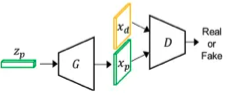
\includegraphics[width=0.85\textwidth]{Figures/GANS.png}
    \caption{Integración de componente adversaria: el discriminador distingue entre configuraciones reales y generadas, mientras el generador aprende a producir muestras cada vez más realistas.}
    \label{fig:gans}
\end{figure}

\subsection{Función de Pérdida Multi-Objetivo Completa}

La función objetivo final combina todos los términos anteriores:

\begin{equation}
\mathcal{L}_{total} = \alpha \mathcal{L}_{recon} + \beta \mathcal{L}_{KL} + \gamma \mathcal{L}_{phys} + \delta \mathcal{L}_{GAN} + \eta \mathcal{L}_{cycle}
\end{equation}

donde $\mathcal{L}_{phys} = \lambda_E \mathcal{L}_{energy} + \lambda_{LLG} \mathcal{L}_{LLG}$.

El problema de optimización consiste en encontrar:

\begin{equation}
\{\theta^*, \psi^*, \phi^*, \alpha^*, \beta^*, \gamma^*, \delta^*, \eta^*\} = \arg\min_{\theta,\psi,\phi,\alpha,\beta,\gamma,\delta,\eta} \mathcal{L}_{total}
\end{equation}

sujeto a restricciones de factibilidad física (e.g., $\|\mathbf{m}\| = 1$ en cada punto).

\begin{figure}[H]
    \centering
    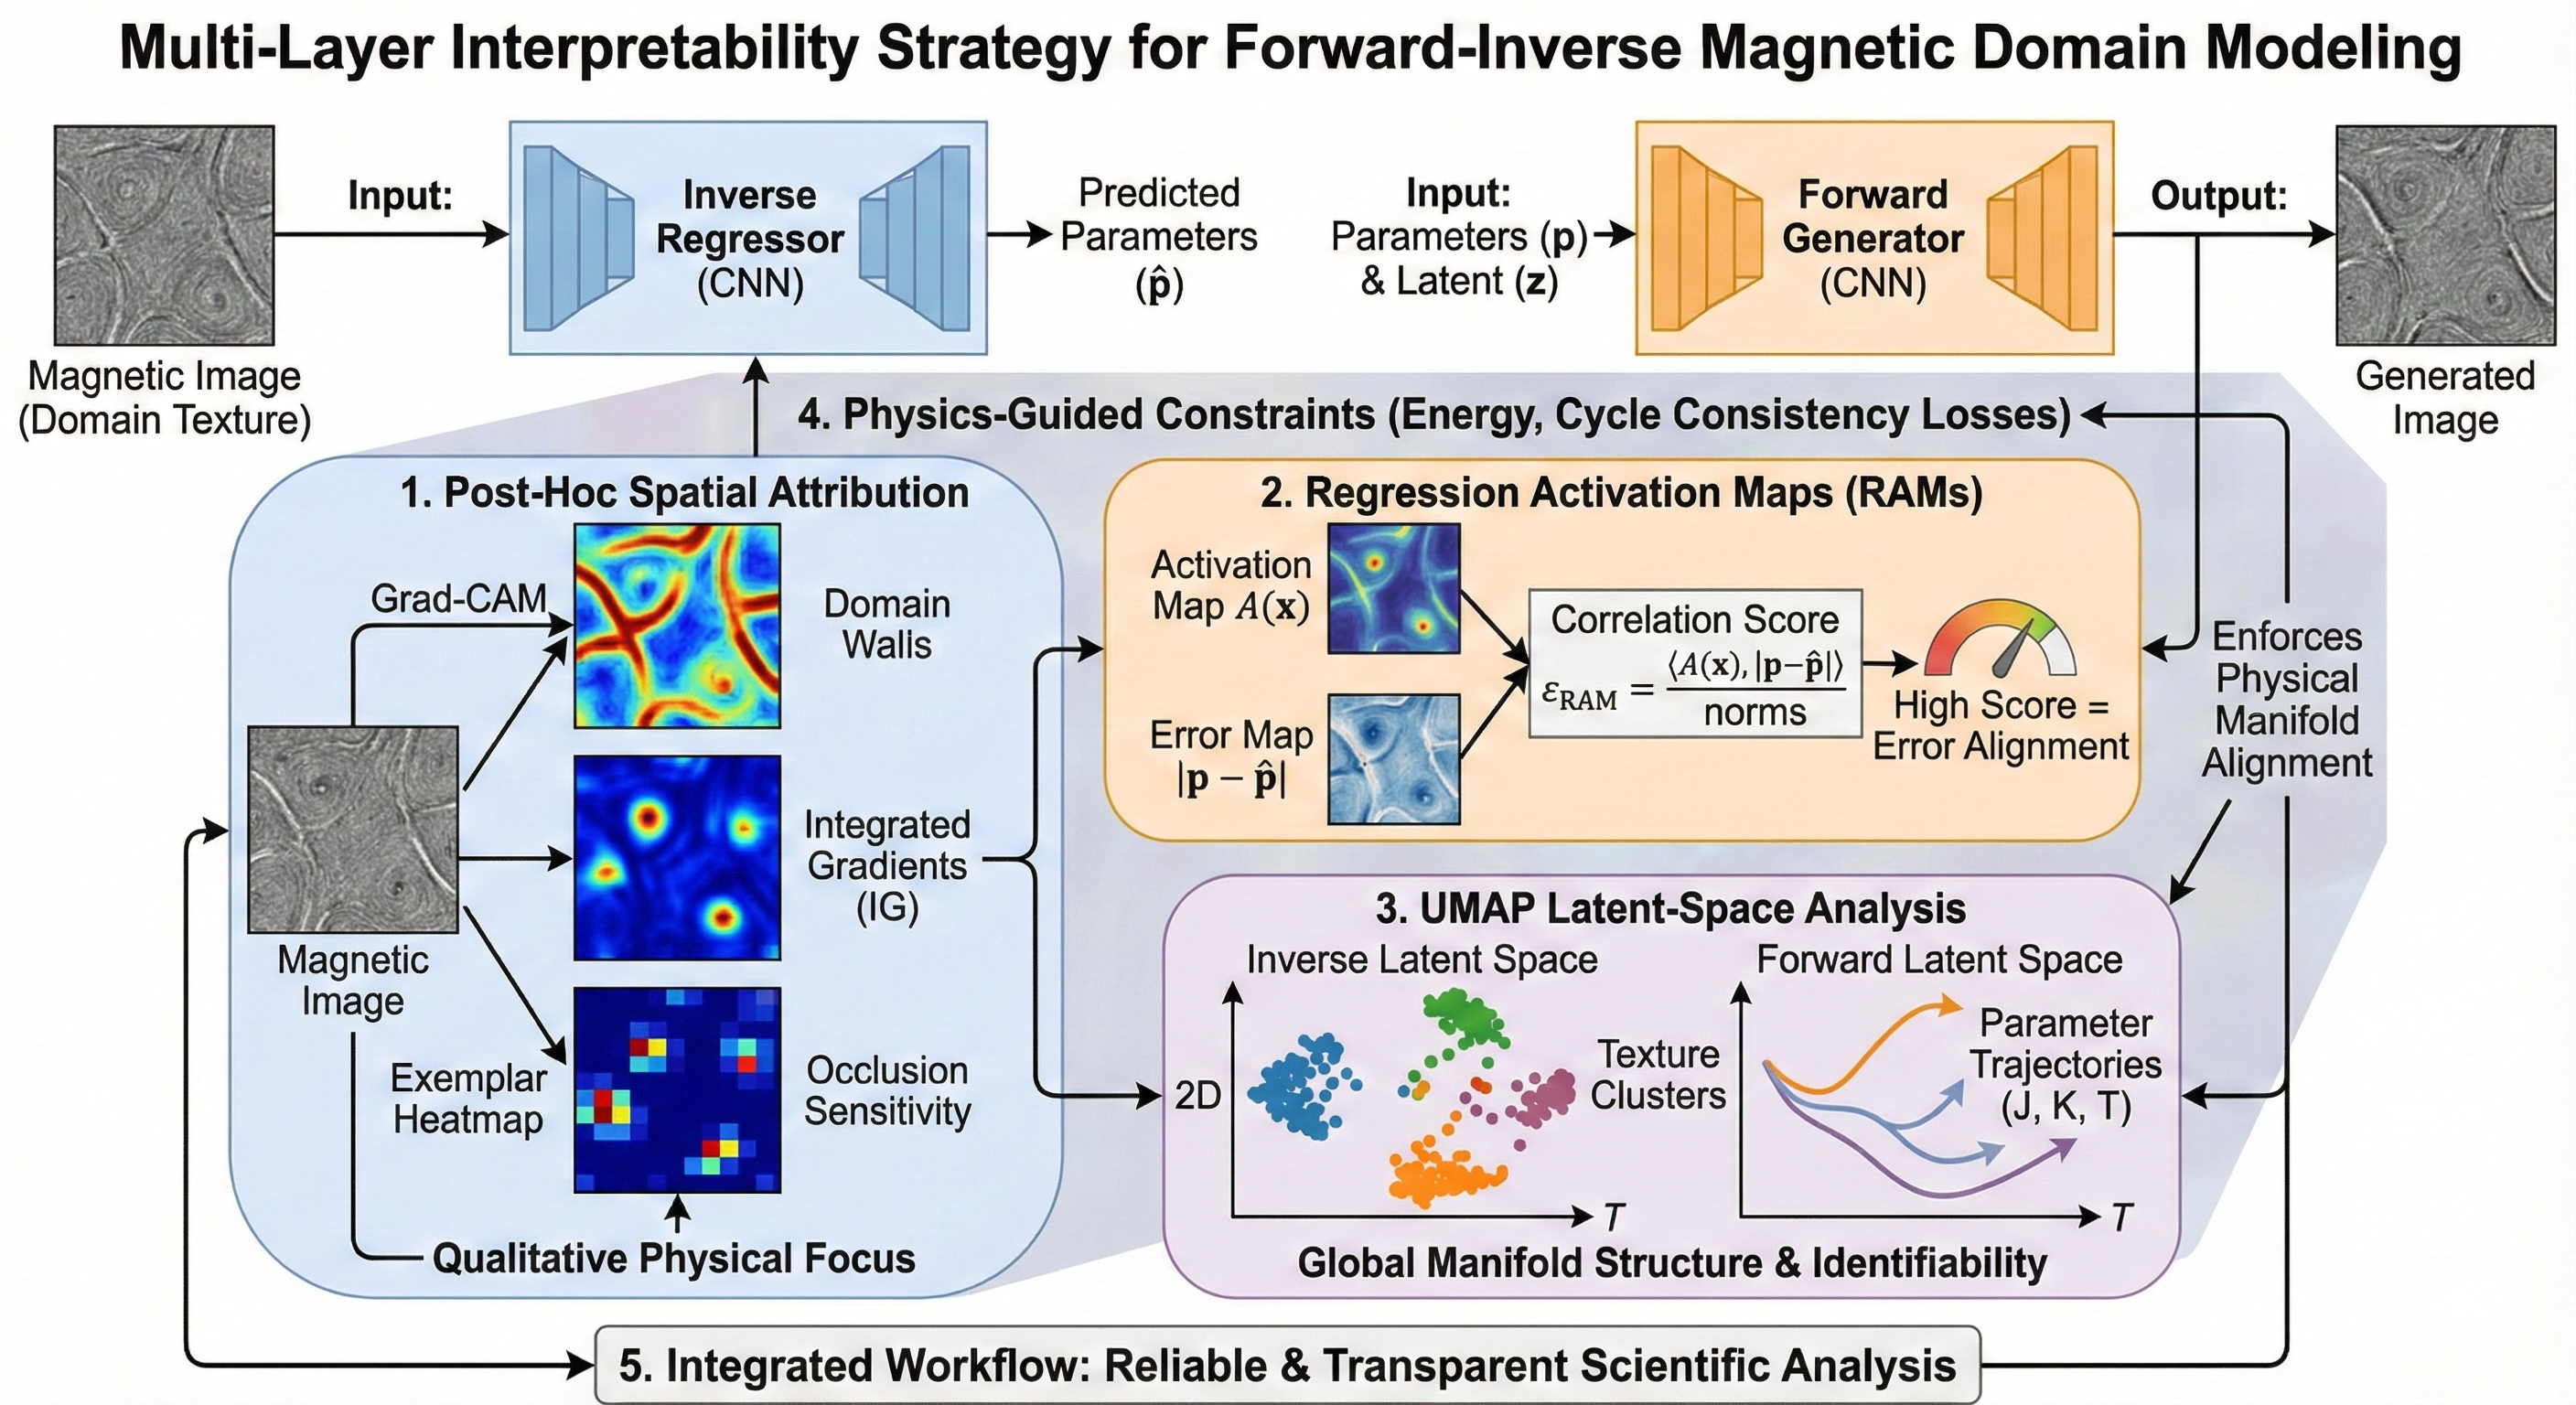
\includegraphics[width=0.95\textwidth]{Figures/Full.png}
    \caption{Arquitectura completa del framework propuesto, integrando cVAE con prior condicional, ciclo-consistencia forward-inverse, regularización física, y componente adversaria para mejoramiento de calidad.}
    \label{fig:full_architecture}
\end{figure}

\section{Configuración Experimental}

\subsection{Bases de Datos}

Se utilizan dos grandes conjuntos de datos sintéticos generados mediante simulaciones Monte Carlo atomísticas:

\begin{enumerate}
    \item \textbf{KDM DATABASE SPINERS}: 164,212 imágenes de configuraciones de espines de $39 \times 39$ píxeles, variando temperatura $T$ y la magnitud de la interacción de Dzyaloshinskii-Moriya $K_{DM}$.

    \item \textbf{MATERIAL SPINNERS DATA}: 54,404 imágenes con la misma resolución, variando temperatura $T$ y parámetros de intercambio de segundo, tercer y cuarto vecinos ($J_{ex2}, J_{ex3}, J_{ex4}$).
\end{enumerate}

\begin{figure}[H]
    \centering
    
\includegraphics[width=0.48\textwidth]{Figures/imagenes_grid.pdf}
    
\includegraphics[width=0.48\textwidth]{Figures/imagenes_grid2.pdf}
    \caption{Ejemplos de configuraciones magnéticas en ambos datasets: (izquierda) KDM DATABASE con texturas quirales inducidas por DMI; (derecha) MATERIAL SPINNERS con estructuras de intercambio variadas.}
    \label{fig:dataset_examples}
\end{figure}

\begin{figure}[H]
    \centering
    
\includegraphics[width=0.48\textwidth]{Figures/distribuciones_parametrosKDM.pdf}
    
\includegraphics[width=0.48\textwidth]{Figures/distribuciones_parametrosTJex2.pdf}
    \caption{Distribuciones de parámetros físicos en ambos datasets. Las variables están muestreadas uniformemente o log-uniformemente para cubrir rangos físicamente relevantes.}
    \label{fig:param_distributions}
\end{figure}

\subsection{Prueba de Concepto 1: cVAE con Prior Condicional}

Se implementó una versión baseline del cVAE usando únicamente la base de datos KDM DATABASE SPINERS, sin incluir las penalidades físicas ($\mathcal{L}_{phys} = 0$) para evaluar la capacidad intrínseca del prior condicional de organizar el espacio latente.

\textbf{Arquitectura}:
\begin{itemize}
    \item \textbf{Encoder}: Capas convolucionales $(64, 128, 256)$ con batch normalization y LeakyReLU, proyección a espacio latente de dimensión $d = 64$
    \item \textbf{Decoder}: Espejo del encoder usando convoluciones transpuestas
    \item \textbf{Prior Network}: MLP de 3 capas $(128, 256, 128)$ que mapea $\mathbf{c} = \{T, K_{DM}\}$ a $\{\mu_\psi, \log\sigma^2_\psi\}$
\end{itemize}

\textbf{Hiperparámetros}:
\begin{itemize}
    \item $\beta = 1.0$ (peso de KL divergence)
    \item Optimizador: Adam con learning rate $= 10^{-4}$
    \item Batch size: 128
    \item Épocas: 100
\end{itemize}

\textbf{Resultados}:

\begin{figure}[H]
    \centering
    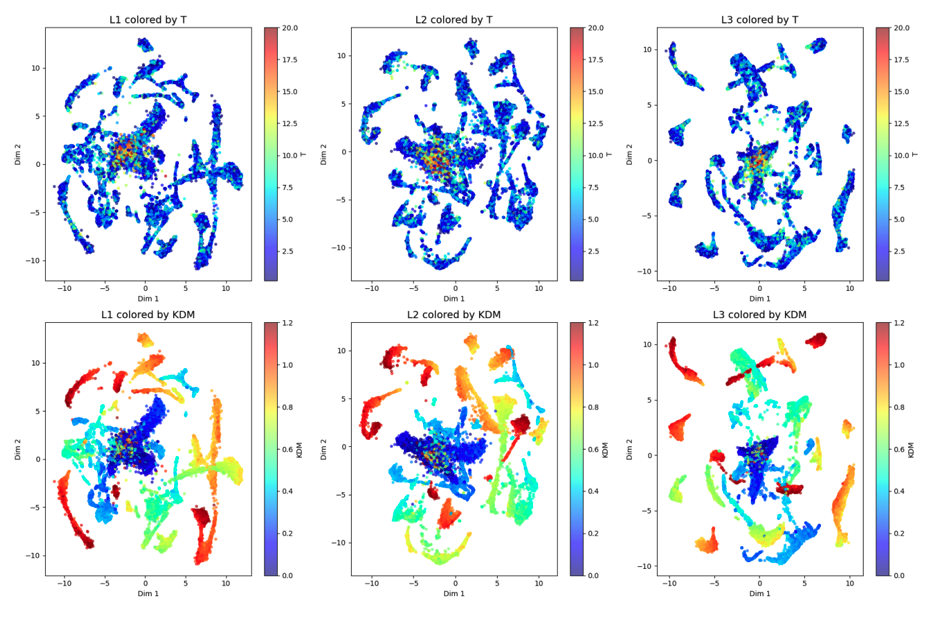
\includegraphics[width=0.48\textwidth]{Figures/UmapDirectTKDM.png}
    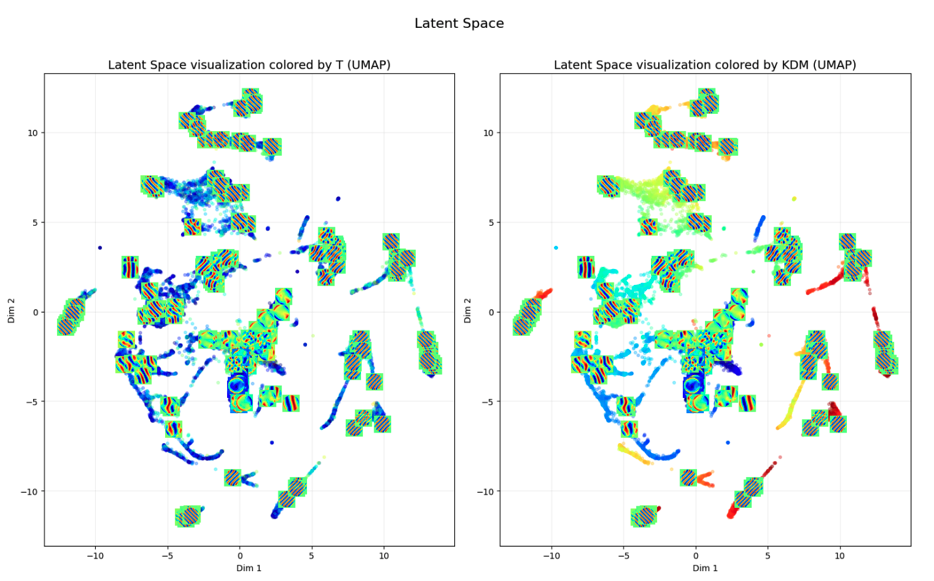
\includegraphics[width=0.48\textwidth]{Figures/UmapDirect.png}
    \caption{Proyecciones UMAP del espacio latente: (izquierda) coloreado por temperatura y KDM mostrando gradientes suaves; (derecha) con imágenes de dominios superpuestas demostrando agrupamiento según características topológicas.}
    \label{fig:umap_results}
\end{figure}

Las visualizaciones UMAP revelan que el prior condicional logra organizar el espacio latente según los parámetros físicos incluso sin restricciones de energía explícitas. Se observan:
\begin{itemize}
    \item Gradientes continuos correspondientes a variaciones de $T$ y $K_{DM}$
    \item Agrupamiento de configuraciones morfológicamente similares (vórtices, paredes de dominio, estructuras quirales)
    \item Separación clara entre regímenes de baja y alta temperatura
\end{itemize}

\begin{figure}[H]
    \centering
    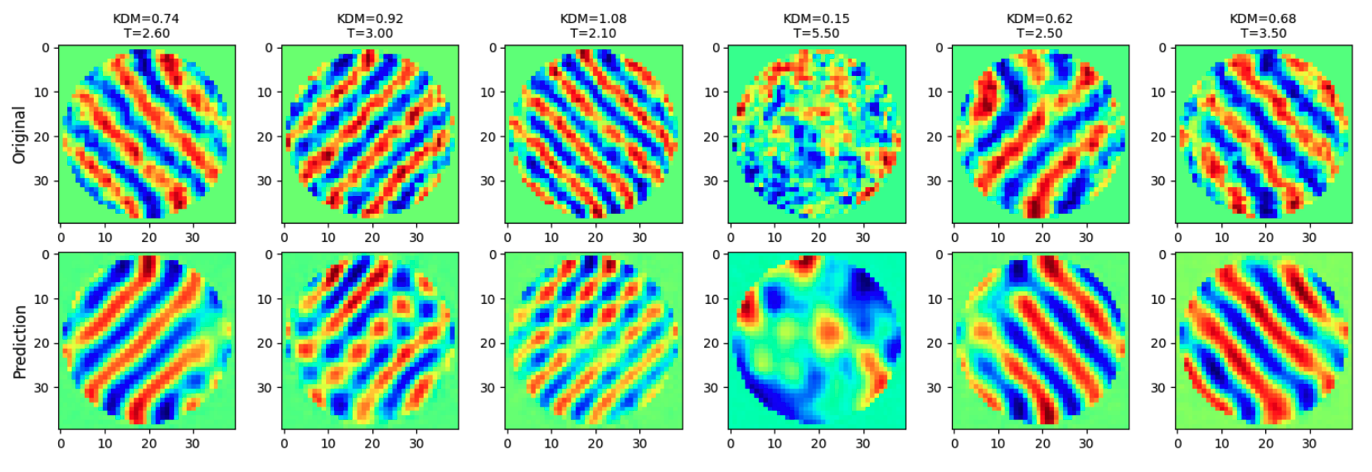
\includegraphics[width=0.85\textwidth]{Figures/Generation.png}
    \caption{Comparación entre configuraciones reales (filas superiores) y reconstrucciones del cVAE (filas inferiores). El modelo captura correctamente las características topológicas principales (núcleos de vórtices, paredes de dominio, efectos de borde) con desviaciones menores en detalles finos.}
    \label{fig:reconstructions}
\end{figure}

\textbf{Limitaciones identificadas}:
\begin{enumerate}
    \item \textbf{Hiperparámetros no optimizados}: Los valores fueron seleccionados manualmente. Se requiere optimización bayesiana sistemática.

    \item \textbf{Invariancia geométrica}: Las configuraciones magnéticas son invariantes a rotaciones, traslaciones y reflexiones. Dos estados que difieren solo en una transformación rígida son físicamente equivalentes, pero MSE les asigna alta disimilitud. Se necesitan métricas invariantes basadas en descriptores topológicos o energía.

    \item \textbf{Ausencia de restricciones físicas}: Sin $\mathcal{L}_{phys}$, el modelo puede generar estados de alta energía o dinámicamente inconsistentes.
\end{enumerate}

\subsection{Prueba de Concepto 2: Optimización Bayesiana Multi-Objetivo con VAE+GAN}

Para validar la viabilidad de optimización bayesiana en el contexto de modelos generativos con múltiples objetivos conflictivos, se realizó un experimento simplificado usando una arquitectura VAE+GAN entrenada sobre los datasets Fashion-MNIST y MNIST.

\subsubsection{Motivación y Simplificación del Problema}

Antes de aplicar optimización bayesiana multi-objetivo al problema completo de dominios magnéticos con la función de pérdida completa:

\begin{equation}
\mathcal{L}_{total} = \alpha \mathcal{L}_{recon} + \beta \mathcal{L}_{KL} + \gamma \mathcal{L}_{phys} + \delta \mathcal{L}_{GAN} + \eta \mathcal{L}_{cycle}
\end{equation}

se diseñó una prueba de concepto con una versión reducida que conserva la naturaleza multi-objetivo pero en un escenario más simple:

\begin{equation}
\mathcal{L}_{simple} = w_{rec} \mathcal{L}_{rec} + \beta \mathcal{L}_{KL} + w_{adv} \mathcal{L}_{GAN}
\end{equation}

donde:
\begin{itemize}
    \item $\mathcal{L}_{rec}$: Error de reconstrucción (MSE píxel a píxel)
    \item $\mathcal{L}_{KL}$: Divergencia KL entre distribución del encoder y prior gaussiano
    \item $\mathcal{L}_{GAN}$: Pérdida adversaria del discriminador
    \item $w_{rec}, \beta, w_{adv}$: Hiperparámetros a optimizar
\end{itemize}

Esta simplificación permite:
\begin{enumerate}
    \item Tiempos de entrenamiento significativamente menores ($\sim$5 minutos por configuración vs. varias horas)
    \item Mayor número de evaluaciones en el proceso de optimización bayesiana
    \item Validación del concepto sin la complejidad adicional de restricciones físicas
\end{enumerate}

\subsubsection{Arquitectura del Modelo}

\textbf{Encoder}:
\begin{itemize}
    \item Entrada: Imágenes $28 \times 28$ en escala de grises
    \item Capas convolucionales: Conv2d(1$\to$32, kernel=4, stride=2) $\to$ Conv2d(32$\to$64, kernel=4, stride=2)
    \item Activación: LeakyReLU($\alpha=0.2$)
    \item Proyección a espacio latente: FC(64$\times$7$\times$7 $\to$ 128) $\to$ FC(128 $\to$ $z_{dim}$)
    \item Salida: $\mu_z$ y $\log\sigma^2_z$ (dimensión latente: 16 o 32)
\end{itemize}

\textbf{Decoder (Generador)}:
\begin{itemize}
    \item Entrada: Vector latente $z \sim \mathcal{N}(\mu_z, \sigma^2_z)$
    \item Capas densas: FC($z_{dim}$ $\to$ 128) $\to$ FC(128 $\to$ 64$\times$7$\times$7)
    \item Capas deconvolucionales: ConvTranspose2d(64$\to$32, kernel=4, stride=2) $\to$ ConvTranspose2d(32$\to$1, kernel=4, stride=2)
    \item Activación final: Sigmoid
\end{itemize}

\textbf{Discriminador}:
\begin{itemize}
    \item Entrada: Imagen real o generada $28 \times 28$
    \item Capas convolucionales: Conv2d(1$\to$32, kernel=4, stride=2) $\to$ Conv2d(32$\to$64, kernel=4, stride=2)
    \item Clasificador: FC(64$\times$7$\times$7 $\to$ 1)
    \item Activación final: Sigmoid (probabilidad de imagen real)
\end{itemize}

\subsubsection{Formulación Multi-Objetivo}

El problema de optimización consiste en encontrar valores óptimos de $\{w_{rec}, \beta, w_{adv}\}$ que minimicen simultáneamente tres funciones objetivo conflictivas:

\begin{equation}
\begin{aligned}
f_1(w_{rec}, \beta, w_{adv}) &= 1 - \text{SSIM}(\text{real}, \text{recon}) \quad \text{(calidad perceptual)} \\
f_2(w_{rec}, \beta, w_{adv}) &= \text{MSE}(\text{real}, \text{recon}) \quad \text{(fidelidad de reconstrucción)} \\
f_3(w_{rec}, \beta, w_{adv}) &= \overline{D_{KL}[q(z|x) \| p(z)]} \quad \text{(regularización latente)}
\end{aligned}
\end{equation}

\textbf{Conflictos entre objetivos}:
\begin{itemize}
    \item Aumentar $\beta$ mejora $f_3$ (distribución latente más regular) pero deteriora $f_1$ y $f_2$ (peor reconstrucción)
    \item Aumentar $w_{rec}$ mejora $f_2$ (menor MSE) pero puede sacrificar $f_1$ (detalles perceptuales)
    \item Aumentar $w_{adv}$ mejora $f_1$ (mejor calidad visual) pero introduce inestabilidad en el entrenamiento
\end{itemize}

\subsubsection{Protocolo de Optimización con Optuna}

Se utilizó el framework Optuna con un sampler TPE (Tree-structured Parzen Estimator) para optimización bayesiana multi-objetivo:

\textbf{Espacio de búsqueda}:
\begin{itemize}
    \item $w_{rec} \in [0.1, 10]$ (escala logarítmica)
    \item $\beta \in [0.0, 5.0]$ (escala lineal)
    \item $w_{adv} \in [0.0, 2.0]$ (escala lineal)
\end{itemize}

\textbf{Configuración de optimización}:
\begin{itemize}
    \item Número de trials: 50
    \item Épocas por trial: 5 (para prueba rápida; 15 para configuraciones finales)
    \item Dataset: Fashion-MNIST (60,000 imágenes de entrenamiento)
    \item Batch size: 128
    \item Optimizador: Adam ($lr = 10^{-3}$)
\end{itemize}

\subsubsection{Resultados: Frontera de Pareto y Análisis}

\begin{figure}[H]
    \centering
    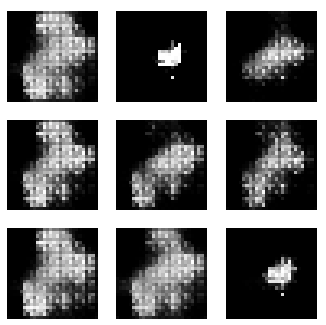
\includegraphics[width=0.85\textwidth]{Figures/OriginalEstimation.png}
    \caption{Estimación inicial con hiperparámetros manuales: las reconstrucciones presentan borrosidad excesiva, pérdida de detalles finos, y distribución latente colapsada ($\beta$ muy bajo). SSIM$\approx$0.72, MSE$\approx$0.035, KL$\approx$0.8.}
    \label{fig:original_estimation}
\end{figure}

\begin{figure}[H]
    \centering
    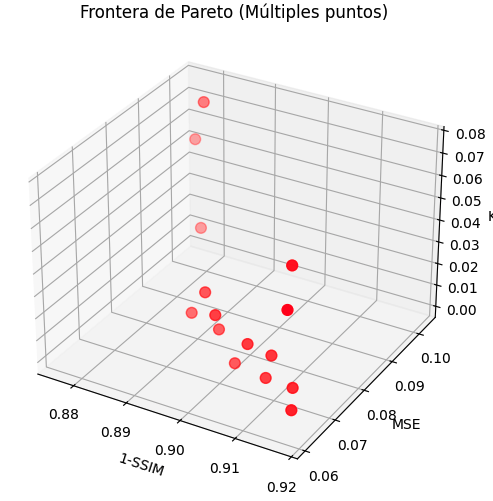
\includegraphics[width=0.9\textwidth]{Figures/FronteraParetos.png}
    \caption{Frontera de Pareto obtenida tras 50 trials de optimización bayesiana. Cada punto representa una configuración de hiperparámetros no-dominada. Se identificaron 12 soluciones Pareto-óptimas distribuidas a lo largo de diferentes trade-offs.}
    \label{fig:pareto_frontier}
\end{figure}

La frontera de Pareto (Figura \ref{fig:pareto_frontier}) revela tres regímenes claramente diferenciados:

\begin{enumerate}
    \item \textbf{Régimen de alta fidelidad}: $w_{rec} \approx 8{-}10$, $\beta \approx 0.5{-}1.0$, $w_{adv} \approx 0.1{-}0.3$
    \begin{itemize}
        \item Minimiza $f_2$ (MSE $\approx$ 0.018)
        \item $f_1$ moderado (SSIM $\approx$ 0.85)
        \item $f_3$ alto (KL $\approx$ 3.2, distribución latente irregular)
    \end{itemize}

    \item \textbf{Régimen balanceado}: $w_{rec} \approx 3{-}5$, $\beta \approx 1.5{-}2.5$, $w_{adv} \approx 0.5{-}0.8$
    \begin{itemize}
        \item Balance óptimo entre todos los objetivos
        \item SSIM $\approx$ 0.88, MSE $\approx$ 0.024, KL $\approx$ 1.8
        \item Mejor compromiso para aplicaciones generales
    \end{itemize}

    \item \textbf{Régimen de calidad perceptual}: $w_{rec} \approx 1{-}2$, $\beta \approx 3{-}4$, $w_{adv} \approx 1.2{-}1.8$
    \begin{itemize}
        \item Minimiza $f_1$ (SSIM $\approx$ 0.92)
        \item $f_2$ ligeramente peor (MSE $\approx$ 0.031)
        \item $f_3$ bajo (KL $\approx$ 1.2, distribución latente suave)
    \end{itemize}
\end{enumerate}

\begin{figure}[H]
    \centering
    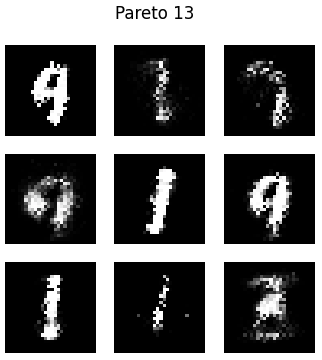
\includegraphics[width=0.48\textwidth]{Figures/UsoPareto1.png}
    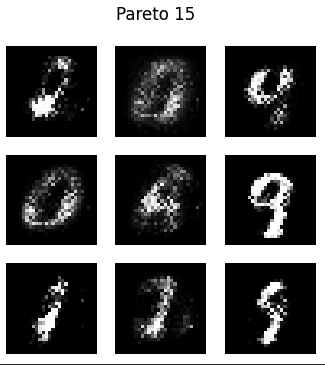
\includegraphics[width=0.48\textwidth]{Figures/UsoPareto2.png}
    \caption{Reconstrucciones usando dos puntos de la frontera de Pareto: (izquierda) configuración de alta fidelidad con detalles finos preservados pero ruido; (derecha) configuración de calidad perceptual con imágenes suaves y visualmente agradables pero menor precisión píxel a píxel.}
    \label{fig:pareto_usage}
\end{figure}

\subsubsection{Implicaciones para el Problema Completo}

Los hallazgos de esta prueba de concepto validan la estrategia de optimización bayesiana multi-objetivo para el problema completo de dominios magnéticos:

\begin{enumerate}
    \item \textbf{No-unicidad fundamental}: Existen múltiples configuraciones de hiperparámetros igualmente válidas según preferencias de trade-off. La búsqueda de un ``mejor'' conjunto único de hiperparámetros es mal planteada.

    \item \textbf{Eficiencia de búsqueda}: TPESampler converge a la frontera de Pareto en $\sim$30-40 trials, significativamente más eficiente que grid search ($> 1000$ evaluaciones para resolución comparable).

    \item \textbf{Selección informada}: La visualización de la frontera permite al usuario seleccionar configuraciones según necesidades específicas (e.g., priorizar consistencia física vs. calidad visual).

    \item \textbf{Escalabilidad}: El framework Optuna soporta optimización distribuida y búsqueda de arquitectura neural (NAS), permitiendo explorar simultáneamente hiperparámetros de pérdida y arquitectura de redes.
\end{enumerate}

\textbf{Trabajo futuro inmediato}: Extender este protocolo al problema completo con $\mathcal{L}_{total}$ incluyendo penalidades físicas, usando métricas de evaluación invariantes a transformaciones geométricas, y diseñando funciones de adquisición Pareto-aware para acelerar la exploración de regiones críticas de la frontera.

\section{Conclusiones Parciales}

Este trabajo ha establecido las bases para abordar la caracterización de dominios magnéticos nanoscópicos como un problema de optimización multi-objetivo. Las pruebas de concepto realizadas validan tanto los componentes del framework propuesto como la metodología de optimización bayesiana:

\begin{enumerate}
    \item \textbf{Viabilidad del cVAE con prior condicional}: El modelo organiza efectivamente el espacio latente según parámetros físicos, logrando gradientes continuos y agrupamiento morfológico incluso sin restricciones de energía explícitas.

    \item \textbf{Validación de optimización bayesiana multi-objetivo}: El experimento simplificado con VAE+GAN sobre Fashion-MNIST demostró que:
    \begin{itemize}
        \item Optuna con TPESampler converge eficientemente a la frontera de Pareto en $\sim$30-40 trials
        \item Existen múltiples configuraciones de hiperparámetros igualmente válidas según diferentes trade-offs
        \item La visualización de la frontera permite selección informada según prioridades específicas
    \end{itemize}

    \item \textbf{Identificación de limitaciones críticas}:
    \begin{itemize}
        \item Los hiperparámetros $\{\alpha, \beta, \gamma, \delta, \eta\}$ determinan trade-offs fundamentales entre objetivos conflictivos
        \item No existe una métrica escalar única que capture todos los aspectos de calidad
        \item Las métricas píxel a píxel (MSE) son inadecuadas para configuraciones invariantes a transformaciones geométricas
    \end{itemize}
\end{enumerate}

\textbf{Próximos pasos}: La siguiente fase del proyecto aplicará el protocolo validado de optimización bayesiana multi-objetivo al problema completo con $\mathcal{L}_{total}$, incorporando:

\begin{itemize}
    \item Métricas de evaluación invariantes a rotaciones y traslaciones (descriptores topológicos, energía micromagnética)
    \item Restricciones físicas explícitas ($\mathcal{L}_{phys}$) en el proceso de optimización
    \item Exploración simultánea de hiperparámetros de pérdida y arquitectura de redes (Neural Architecture Search)
    \item Funciones de adquisición Pareto-aware para acelerar exploración de regiones críticas
    \item Validación sobre datos experimentales mediante técnicas de adaptación de dominio
\end{itemize}

% \bibliographystyle{plain}
% \bibliography{references}

\end{document}
